\chapter{Organische moleculen: skeletten en namen}\label{ch:g11:organic-skeletons}

Een wegwerpaansteker bevat butaan, vloeibaar onder druk; het busje van
een kampeerbrander dat mee de besneeuwde berg op gaat, bevat propaan, of
een \omterm{def:g6:pure-substances-and-mixtures:mixture}{mengsel} dat er rijker aan is. Beide bestaan uit niets anders dan
koolstof- en waterstofatomen, en beide horen bij een enorme familie: de
\omterm{def:g7:atoms-and-molecules:molecule}{moleculen} die gebouwd zijn op een skelet van koolstofatomen. Er zijn er
miljoenen van bekend. Om erover te praten, hebben scheikundigen manieren
nodig om ze snel te tekenen en ze zonder dubbelzinnigheid een naam te
geven.

\begin{recall}
Koolstof vormt vier \omterm{def:g10:lewis-and-shape:covalent-bond}{covalente bindingen} en waterstof één; rond een
koolstofatoom met vier enkele bindingen wijzen de bindingen naar de
hoekpunten van een tetraëder, onder ongeveer \ang{109.5}
(\cref{ch:g10:lewis-and-shape}).
\end{recall}

\begin{omfigure}
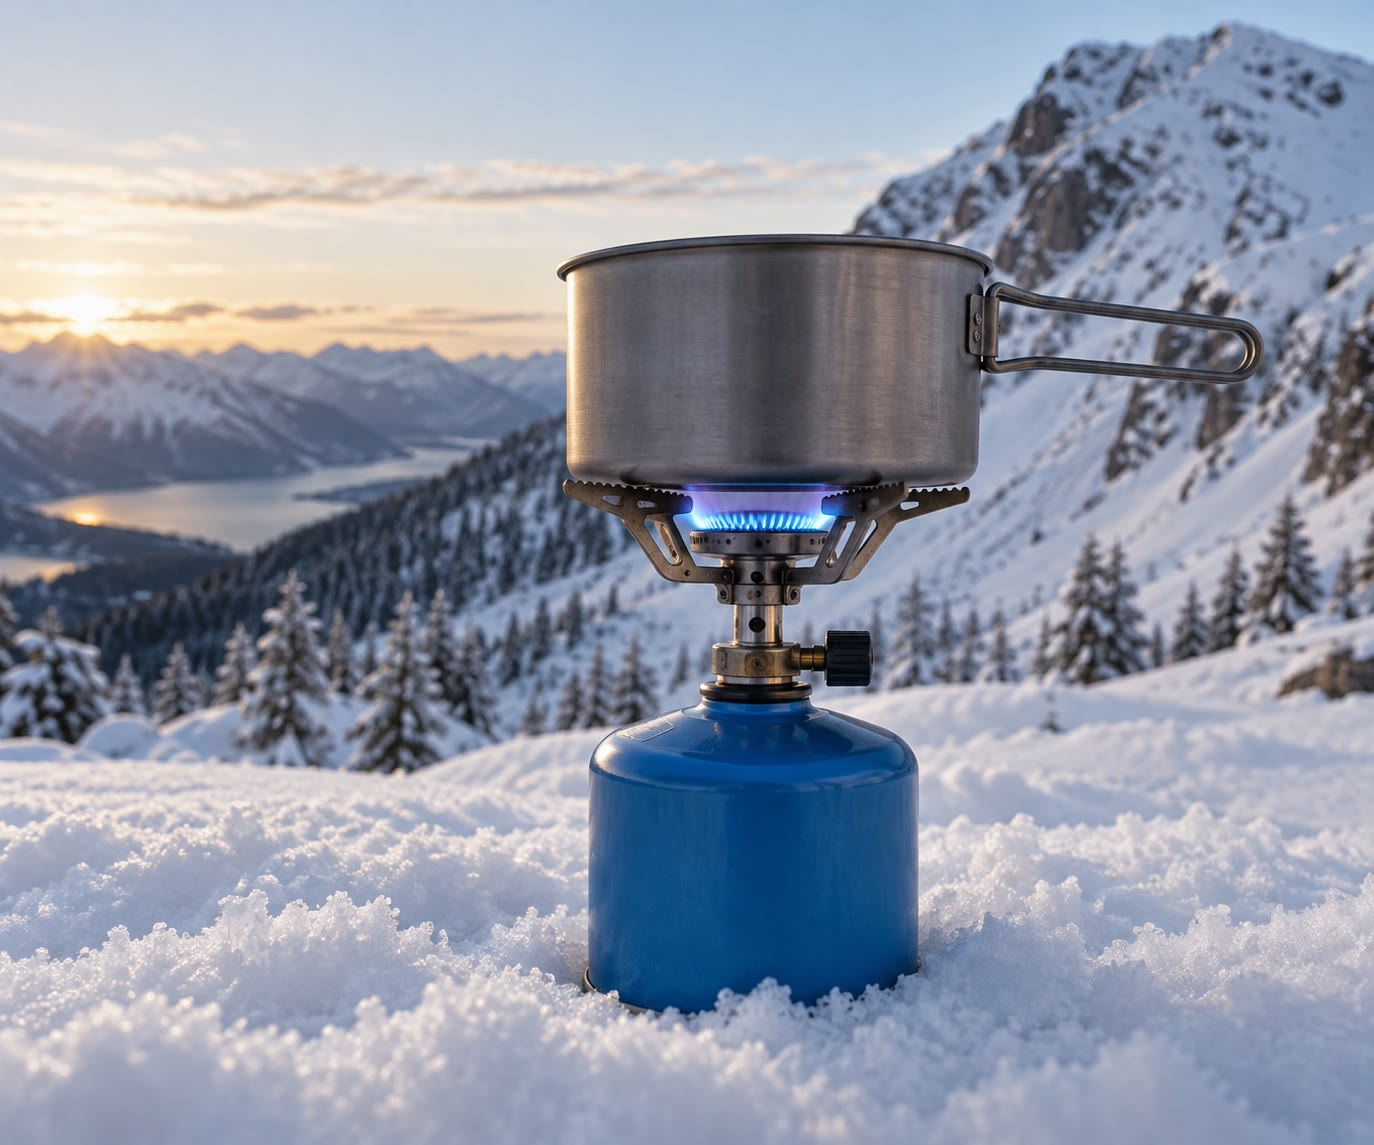
\includegraphics[width=0.48\linewidth]{images/book1/ai/g11-camping-cartridge.jpg}

{\small Een kampeerbrander in de sneeuw, die een gas uit koolstof en
waterstof verbrandt.}
\end{omfigure}

\section{Formules van organische moleculen}

\begin{definition}[Organische verbinding]\label{def:g11:organic-skeletons:organic}
Een \emph{organische verbinding}\index{organische verbinding} is een
verbinding waarvan de \omterm{def:g7:atoms-and-molecules:molecule}{moleculen} gebouwd zijn op een skelet van
koolstofatomen die aan elkaar en aan waterstofatomen gebonden zijn,
eventueel met andere \omterm{def:g7:atoms-and-molecules:atom}{atomen} zoals zuurstof en stikstof.
(Koolstofdioxide, koolstofmono-oxide en de carbonaten worden er
traditioneel niet toe gerekend.)
\end{definition}

\begin{definition}[Vier soorten formules]\label{def:g11:organic-skeletons:formulas}
Een \omterm{def:g7:atoms-and-molecules:molecule}{molecuul} kun je op vier manieren opschrijven:
\begin{itemize}
  \item de \emph{molecuulformule}\index{molecuulformule} geeft alleen het
        aantal \omterm{def:g7:atoms-and-molecules:atom}{atomen} van elk element, zoals \ce{C4H10};
  \item de \emph{structuurformule}\index{structuurformule} toont elk \omterm{def:g7:atoms-and-molecules:atom}{atoom}
        en elke binding;
  \item de \emph{beknopte structuurformule}\index{beknopte structuurformule}
        toont de bindingen tussen koolstofatomen en groepeert de
        waterstofatomen bij hun koolstof, zoals \ce{CH3-CH2-CH2-CH3};
  \item de \emph{skeletformule}\index{skeletformule} tekent alleen de
        bindingen van het koolstofskelet als een zigzag: elk uiteinde en
        elk hoekpunt is een koolstofatoom, de waterstofatomen aan koolstof
        worden niet getekend, en elk ander \omterm{def:g7:atoms-and-molecules:atom}{atoom} (met zijn
        waterstofatomen) wordt opgeschreven.
\end{itemize}
\end{definition}

\begin{omfigure}
\setchemfig{atom sep=1.45em}
\renewcommand{\arraystretch}{1.6}
\small
\begin{tabular}{@{}l@{\quad}c@{\quad}c@{}}
 & butaan & 2-methylpropaan \\
\omterm{def:g7:atoms-and-molecules:molecule}{molecuul} & \ce{C4H10} & \ce{C4H10} \\[4pt]
structuur &
\chemfig{H-C(-[2]H)(-[6]H)-C(-[2]H)(-[6]H)-C(-[2]H)(-[6]H)-C(-[2]H)(-[6]H)-H} &
\chemfig{H-C(-[2]H)(-[6]H)-C(-[6]H)(-[2,1.5]C(-[1]H)(-[3]H)(-[2]H))-C(-[2]H)(-[6]H)-H} \\[10pt]
beknopt & \ce{CH3-CH2-CH2-CH3} &
\chemfig{CH_3-CH(-[6]CH_3)-CH_3} \\[14pt]
skelet & \chemfig{-[:30]-[:-30]-[:30]} & \chemfig{-[:30](-[:90])-[:-30]} \\
\end{tabular}

{\small De vier formules van butaan en van 2-methylpropaan. In de
\omterm{def:g11:organic-skeletons:formulas}{skeletformules} is elk uiteinde en elk hoekpunt van de lijnen een
koolstofatoom: vier in elk.}
\end{omfigure}


\begin{example}[Een skeletformule lezen]\label{ex:g11:organic-skeletons:reading}
In de \omterm{def:g11:organic-skeletons:formulas}{skeletformule} van butaan heeft de zigzag twee uiteinden en twee
hoekpunten: vier koolstofatomen. Elk eindkoolstofatoom heeft één
getekende binding, dus draagt het drie waterstofatomen (\ce{CH3}); elk
hoekpunt heeft twee getekende bindingen, dus draagt het er twee
(\ce{CH2}). Elk koolstofatoom heeft in totaal vier bindingen, wat weer
\ce{C4H10} geeft.
\end{example}

\section{Koolstofketens}

Het koolstofskelet van een \omterm{def:g7:atoms-and-molecules:molecule}{molecuul} kan een \emph{onvertakte} keten
zijn, waarin elk koolstofatoom aan hoogstens twee andere gebonden is,
zoals in butaan; een \emph{vertakte} keten, met minstens één
koolstofatoom dat aan drie of vier andere gebonden is, zoals in
2-methylpropaan; of een \emph{ring}, zoals in cyclohexaan, \ce{C6H12},
waarvan de \omterm{def:g11:organic-skeletons:formulas}{skeletformule} een zeshoek is. Voor ketens gebruik je een
zigzag, omdat de echte bindingen rond elk koolstofatoom hoeken van
ongeveer \ang{109.5} maken, en niet van \ang{180}: een ``rechte'' keten
is in de ruimte in feite een zigzag.

\begin{omfigure}
\setchemfig{atom sep=1.9em}
\begin{tabular}{ccc}
\chemfig{-[:30]-[:-30]-[:30]-[:-30]-[:30]} &
\chemfig{-[:30](-[:90])-[:-30]-[:30](-[:90])-[:-30]} &
\chemfig{*6(------)} \\[4pt]
\small onvertakt: hexaan & \small vertakt: 2,4-dimethylpentaan &
\small ring: cyclohexaan \\
\small \ce{C6H14} & \small \ce{C7H16} & \small \ce{C6H12}
\end{tabular}

{\small Drie koolstofskeletten, in \omterm{def:g11:organic-skeletons:formulas}{skeletformules}.}
\end{omfigure}

\section{Alkanen en hun namen}

\begin{definition}[Alkaan, alkylgroep]\label{def:g11:organic-skeletons:alkane}
Een \emph{alkaan}\index{alkaan} is een verbinding van koolstof en
waterstof waarvan het skelet een keten is (onvertakt of vertakt, geen
ring) met alleen enkele bindingen; de \omterm{def:g11:organic-skeletons:formulas}{molecuulformule} is
\ce{C_{n}H_{2n+2}}. Een \emph{alkylgroep}\index{alkylgroep} is wat er van
een alkaan overblijft als je er één waterstofatoom van afhaalt, zodat het
aan een keten kan vastzitten: methyl \ce{-CH3}, ethyl \ce{-CH2-CH3}.
\end{definition}

\begin{omfigure}
\begin{tabular}{rlcrlc}
\hline
$n$ & naam & formule & $n$ & naam & formule \\
\hline
1 & methaan & \ce{CH4}    & 6  & hexaan & \ce{C6H14} \\
2 & ethaan  & \ce{C2H6}   & 7  & heptaan & \ce{C7H16} \\
3 & propaan & \ce{C3H8}   & 8  & octaan & \ce{C8H18} \\
4 & butaan  & \ce{C4H10}  & 9  & nonaan & \ce{C9H20} \\
5 & pentaan & \ce{C5H12}  & 10 & decaan & \ce{C10H22} \\
\hline
\end{tabular}\par\medskip

{\small De eerste tien onvertakte \omterm{def:g11:organic-skeletons:alkane}{alkanen}. De naam van een keten van $n$
koolstofatomen is steeds de stam gevolgd door \emph{-aan}; de \omterm{def:g11:organic-skeletons:alkane}{alkylgroep}
vervangt \emph{-aan} door \emph{-yl} (methyl, ethyl, propyl\dots).}
\end{omfigure}

\begin{method}[Een alkaan een naam geven]\label{met:g11:organic-skeletons:naming}
\begin{enumerate}
  \item Zoek de langste keten van koolstofatomen: die geeft de stamnaam
        (pentaan, hexaan\dots).
  \item De \omterm{def:g7:atoms-and-molecules:atom}{atomen} die er niet in zitten, vormen \omterm{def:g11:organic-skeletons:alkane}{alkylgroepen} die eraan
        vastzitten, de substituenten.
  \item Nummer de hoofdketen vanaf het uiteinde dat de substituenten de
        laagste nummers geeft.
  \item Schrijf elke substituent met zijn nummer (zijn plaats op de
        keten), in alfabetische volgorde, vóór de stam; herhaalde groepen
        krijgen de voorvoegsels di-, tri-, tetra-, met elk een eigen
        nummer. Nummers worden gescheiden door komma's, nummers en woorden
        door streepjes.
\end{enumerate}
\end{method}

\begin{omfigure}
\begin{tikzpicture}[font=\small, x=0.9cm, y=0.9cm]
  % main chain of 5, zigzag; methyls on C2 and C3
  \coordinate (a1) at (0,0); \coordinate (a2) at (0.87,0.5);
  \coordinate (a3) at (1.73,0); \coordinate (a4) at (2.6,0.5);
  \coordinate (a5) at (3.46,0);
  \coordinate (m2) at (0.87,1.5); \coordinate (m3) at (1.73,-1);
  \draw[line width=1pt] (a1) -- (a2) -- (a3) -- (a4) -- (a5);
  \draw[line width=1pt] (a2) -- (m2); \draw[line width=1pt] (a3) -- (m3);
  \foreach \k in {1,2,3,4,5}
    \node[omDef, font=\footnotesize\bfseries, fill=white, inner sep=1pt]
      at ($(a\k)+(0,-0.32)$) {\k};
  \draw[omProp, thick] (m2) circle (0.28);
  \draw[omProp, thick] (m3) circle (0.28);
  \node[omProp, anchor=west] at ($(m2)+(0.35,0)$) {methyl aan C2};
  \node[omProp, anchor=west] at ($(m3)+(0.35,0)$) {methyl aan C3};
  \node[anchor=west, align=left] at (5,0.3) {langste keten: 5 koolstofatomen,
    \emph{pentaan}\\ genummerd vanaf links: 2 en 3\\ (vanaf rechts: 3
    en 4, hoger)\\ naam: \textbf{2,3-dimethylpentaan}};
\end{tikzpicture}

{\small Een vertakt \omterm{def:g11:organic-skeletons:alkane}{alkaan} een naam geven: de hoofdketen (genummerd), de
substituenten (omcirkeld), de naam.}
\end{omfigure}

\begin{method}[Van een naam naar een skeletformule]\label{met:g11:organic-skeletons:drawing}
\begin{enumerate}
  \item Teken de hoofdketen die bij de stam hoort als een zigzag, en
        nummer de koolstofatomen.
  \item Zet elke substituent op de plaats die zijn nummer aangeeft.
  \item Controleer: tel de koolstofatomen, en kijk of geen enkel
        koolstofatoom meer dan vier bindingen heeft.
\end{enumerate}
\end{method}

\section{Isomeren}

\begin{definition}[Isomeren, structuurisomeren]\label{def:g11:organic-skeletons:isomer}
\emph{Isomeren}\index{isomeren} zijn verschillende verbindingen met
dezelfde \omterm{def:g11:organic-skeletons:formulas}{molecuulformule}.
\emph{Structuurisomeren}\index{structuurisomeren} zijn isomeren waarvan
de \omterm{def:g7:atoms-and-molecules:atom}{atomen} in een andere volgorde aan elkaar gebonden zijn, bijvoorbeeld
met een ander koolstofskelet.
\end{definition}

\begin{proposition}[Isomeren hebben verschillende eigenschappen]\label{prop:g11:organic-skeletons:properties}
% ledger: bp:C4H10, bp:isobutane, bp:C5H12, bp:isopentane, bp:neopentane
\omterm{def:g11:organic-skeletons:isomer}{Structuurisomeren} zijn verschillende stoffen, met verschillende
eigenschappen. Van de alkaanisomeren met een bepaalde formule koken de
sterker vertakte lager: butaan kookt bij ongeveer \qty{0}{\celsius} en
2-methylpropaan bij \qty{-11.7}{\celsius}; pentaan bij
\qty{36.1}{\celsius}, 2-methylbutaan bij \qty{27.8}{\celsius} en
2,2-dimethylpropaan bij \qty{9.5}{\celsius}.
\end{proposition}

\begin{proof}
De waarden zijn gemeten (ledger). Vertakte \omterm{def:g7:atoms-and-molecules:molecule}{moleculen} zijn compacter, met
minder oppervlak dat hun buren raakt: hun \omterm{def:g11:polarity-and-cohesion:van-der-waals}{vanderwaalsbindingen} zijn
zwakker (\cref{ch:g11:polarity-and-cohesion}).
\end{proof}

\begin{omfigure}
\setchemfig{atom sep=2em}
\begin{tabular}{ccc}
\chemfig{-[:30]-[:-30]-[:30]-[:-30]} &
\chemfig{-[:30](-[:90])-[:-30]-[:30]} &
\chemfig{-[:0](-[:90])(-[:-90])-[:0]} \\[24pt]
\small pentaan & \small 2-methylbutaan & \small 2,2-dimethylpropaan \\
\small \qty{36.1}{\celsius} & \small \qty{27.8}{\celsius} &
\small \qty{9.5}{\celsius}
\end{tabular}
\medskip

{\small De drie \omterm{def:g11:organic-skeletons:isomer}{isomeren} van \ce{C5H12} en hun kookpunten: hoe sterker
vertakt, hoe lager.}
\end{omfigure}

\section{Alkanen uit aardolie}

Ruwe aardolie is een \omterm{def:g6:pure-substances-and-mixtures:mixture}{mengsel} van duizenden verbindingen, de meeste
daarvan \omterm{def:g11:organic-skeletons:alkane}{alkanen} met 1 tot meer dan 40 koolstofatomen. In een raffinaderij
wordt ze verhit en stijgen de dampen op door een hoge kolom, die naar
boven toe steeds koeler wordt: elke fractie condenseert op de hoogte
waar de temperatuur bij haar kooktraject past. Gassen (methaan tot
butaan) verlaten de kolom bovenaan, daarna benzine, kerosine, diesel;
zware oliën en bitumen blijven onderaan. Deze gefractioneerde
\omterm{def:g10:chemical-species:distillation}{destillatie} scheidt op kookpunt, dat bij \omterm{def:g11:organic-skeletons:alkane}{alkanen} toeneemt met de lengte
van de keten.

\begin{omfigure}
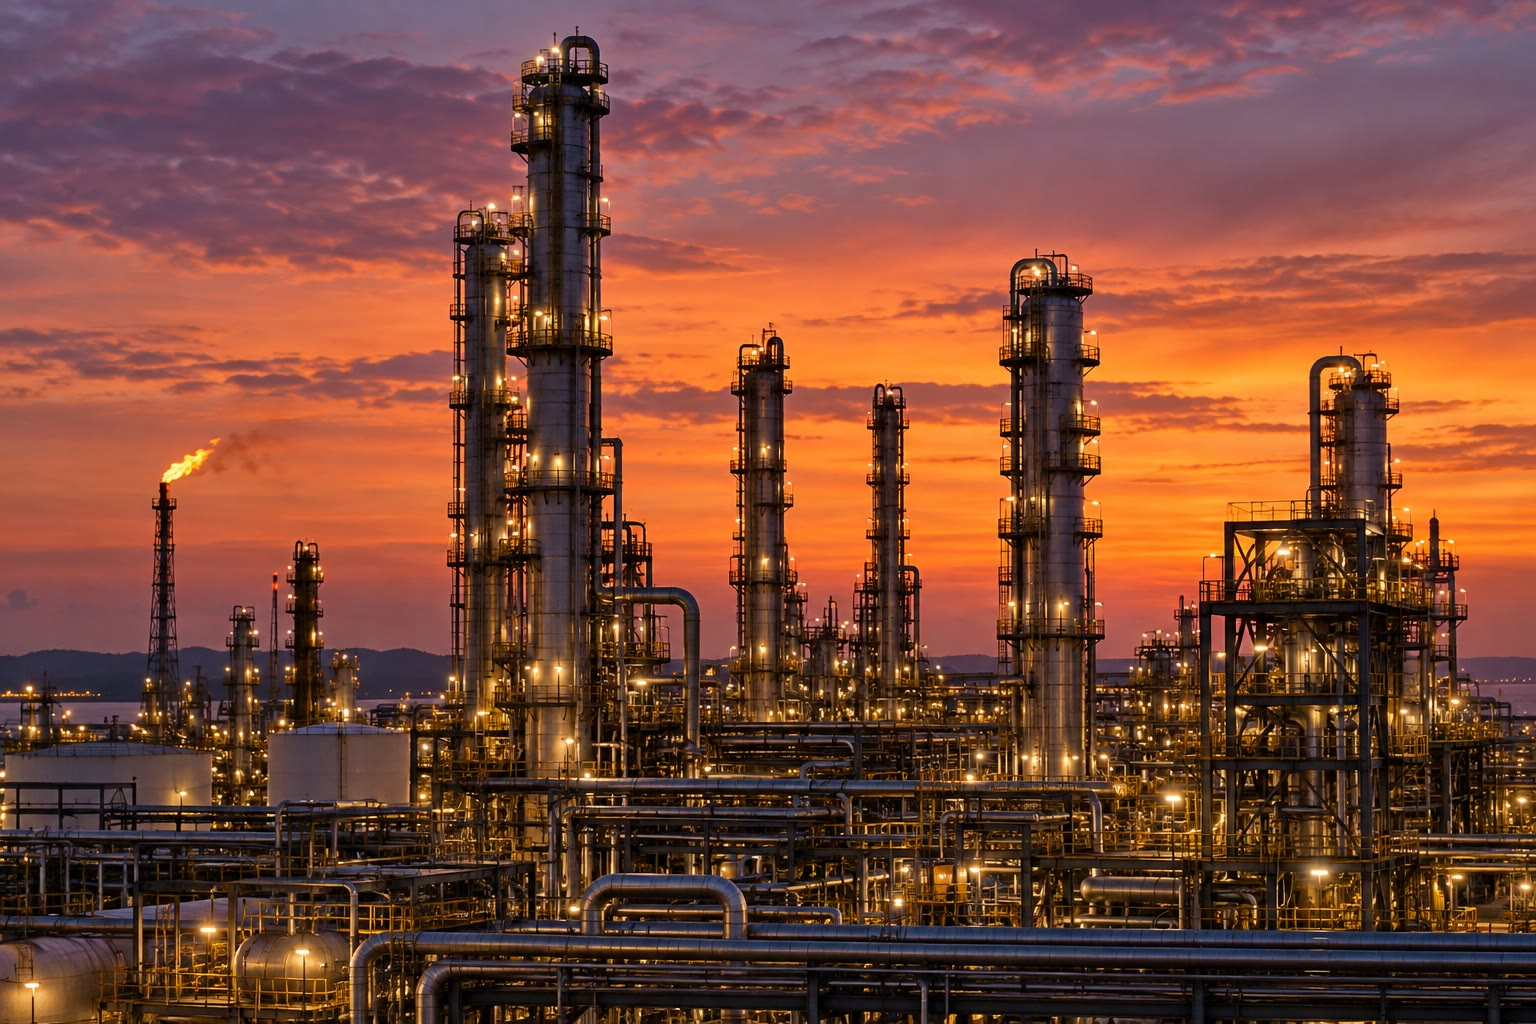
\includegraphics[width=0.52\linewidth]{images/book1/ai/g11-refinery-dusk.jpg}

{\small Destillatiekolommen van een raffinaderij in de schemering.}
\end{omfigure}

\begin{safety}{\ghs[0.66cm]{GHS02}\ghs[0.66cm]{GHS04}\ghs[0.66cm]{GHS07}\ghs[0.66cm]{GHS08}\ghs[0.66cm]{GHS09}}
% ledger: ghs:butane, ghs:pentane
Butaan is een zeer licht ontvlambaar gas, opgeslagen onder druk. Pentaan
is een licht ontvlambare vloeistof; de damp maakt slaperig, het kan de
longen beschadigen als het wordt ingeslikt, en het is giftig voor in het
water levende organismen. Geen vlam bij lichte \omterm{def:g11:organic-skeletons:alkane}{alkanen}; werk in een
zuurkast.
\end{safety}

\section{Oefeningen}


\begin{exercise}[$\star$]\label{exo:g11:organic-skeletons:1}
Geef de \omterm{def:g11:organic-skeletons:formulas}{molecuulformules} van de getekende \omterm{def:g7:atoms-and-molecules:molecule}{moleculen}, en zeg of het
\omterm{def:g11:organic-skeletons:isomer}{isomeren} zijn:
\setchemfig{atom sep=1.6em}
\chemfig{-[:30]-[:-30]-[:30]-[:-30]-[:30]} \quad en \quad
\chemfig{-[:30](-[:90])-[:-30]-[:30]-[:-30]}.
\end{exercise}

\begin{exercise}[$\star$]\label{exo:g11:organic-skeletons:2}
Geef de naam van: \ce{CH3-CH2-CH3}; \ce{CH3-CH2-CH2-CH2-CH2-CH3};
\chemfig{CH_3-CH(-[2]CH_3)-CH_2-CH_3}.
\end{exercise}

\begin{exercise}[$\star$]\label{exo:g11:organic-skeletons:3}
Schrijf de \omterm{def:g11:organic-skeletons:formulas}{beknopte structuurformules} van propaan en van 2-methylpropaan
op, en de \omterm{def:g11:organic-skeletons:formulas}{structuurformule} van ethaan.
\end{exercise}

\begin{exercise}[$\star$]\label{exo:g11:organic-skeletons:4}
Tel de koolstof- en waterstofatomen van elk \omterm{def:g7:atoms-and-molecules:molecule}{molecuul}:
\setchemfig{atom sep=1.6em}
\chemfig{-[:30]-[:-30](-[:-90])-[:30]-[:-30]} \quad en \quad
\chemfig{*6(------)}.
\end{exercise}

\begin{exercise}[$\star$]\label{exo:g11:organic-skeletons:5}
Geef de \omterm{def:g11:organic-skeletons:formulas}{molecuulformule} van het \omterm{def:g11:organic-skeletons:alkane}{alkaan} met 8 koolstofatomen, en het
aantal koolstofatomen van het \omterm{def:g11:organic-skeletons:alkane}{alkaan} met 20 waterstofatomen.
\end{exercise}

\begin{exercise}[$\star\star$]\label{exo:g11:organic-skeletons:6}
Teken de \omterm{def:g11:organic-skeletons:formulas}{skeletformules} van 3-methylhexaan, 2,2-dimethylbutaan en
3-ethylpentaan, en geef hun \omterm{def:g11:organic-skeletons:formulas}{molecuulformules}.
\end{exercise}

\begin{exercise}[$\star\star$]\label{exo:g11:organic-skeletons:7}
Teken de drie \omterm{def:g11:organic-skeletons:isomer}{isomeren} van \ce{C5H12} en geef hun namen.
\end{exercise}

\begin{exercise}[$\star\star$]\label{exo:g11:organic-skeletons:8}
Deze namen zijn fout. Teken elk \omterm{def:g7:atoms-and-molecules:molecule}{molecuul} en geef de juiste naam:
2-ethylbutaan; 4-methylpentaan; 1-methylbutaan.
\end{exercise}

\begin{exercise}[$\star\star$]\label{exo:g11:organic-skeletons:9}
Zet de \omterm{def:g11:organic-skeletons:isomer}{isomeren} van \ce{C5H12} met de figuur op volgorde van kookpunt, en
verklaar de volgorde.
\end{exercise}

\begin{exercise}[$\star\star$]\label{exo:g11:organic-skeletons:10}
Cyclohexaan is \ce{C6H12} en hexaan \ce{C6H14}. Verklaar de twee
ontbrekende waterstofatomen. Zijn de twee verbindingen \omterm{def:g11:organic-skeletons:isomer}{isomeren}? Is
cyclohexaan een \omterm{def:g11:organic-skeletons:alkane}{alkaan}?
\end{exercise}

\begin{exercise}[$\star\star$]\label{exo:g11:organic-skeletons:11}
Welke van propaan, butaan, 2-methylpropaan en cyclobutaan (\ce{C4H8},
een ring van vier koolstofatomen) zijn \omterm{def:g11:organic-skeletons:isomer}{isomeren} van elkaar?
\end{exercise}

\begin{exercise}[$\star\star\star$]\label{exo:g11:organic-skeletons:12}
Teken de vijf \omterm{def:g11:organic-skeletons:isomer}{isomeren} van \ce{C6H14} en geef hun namen.
\end{exercise}

\begin{exercise}[$\star\star\star$]\label{exo:g11:organic-skeletons:13}
Stel je een onvertakt \omterm{def:g11:organic-skeletons:alkane}{alkaan} voor als een lange zigzag en een sterk
vertakt \omterm{def:g11:organic-skeletons:alkane}{alkaan} als een bal. Leg met dit beeld uit waarom vertakking het
kookpunt van \omterm{def:g11:organic-skeletons:isomer}{isomeren} verlaagt.
\end{exercise}

\begin{exercise}[$\star\star\star$]\label{exo:g11:organic-skeletons:14}
Geef de naam van het \omterm{def:g11:organic-skeletons:alkane}{alkaan}
\begin{center}
\chemfig{CH_3-CH(-[2]CH_3)-CH_2-C(-[2]CH_3)(-[6]CH_3)-CH_2-CH_3}
\end{center}
\end{exercise}

\begin{exercise}[$\star\star\star$]\label{exo:g11:organic-skeletons:15}
De referentieverbinding voor benzine, ``isooctaan'', is
2,2,4-trimethylpentaan. Teken de \omterm{def:g11:organic-skeletons:formulas}{skeletformule}, controleer dat het een
\omterm{def:g11:organic-skeletons:isomer}{isomeer} is van octaan, en schrijf de \omterm{def:g11:organic-skeletons:formulas}{beknopte structuurformule} op.
\end{exercise}

\section{Probleem: Aanstekergas}

\begin{problem}[{Weekendprobleem --- hoeveel verschillende \omterm{def:g11:organic-skeletons:alkane}{alkanen} hebben
de formule \ce{C7H16}?}]
\label{pb:g11:organic-skeletons:1}
% ledger: bp:C3H8, bp:C4H10, bp:isobutane
Een aansteker bevat butaan; een busje voor kamperen in de winter bevat een
\omterm{def:g6:pure-substances-and-mixtures:mixture}{mengsel} dat rijker is aan propaan of aan 2-methylpropaan. Butaan kookt
bij ongeveer \qty{0}{\celsius}, 2-methylpropaan bij \qty{-11.7}{\celsius}
en propaan bij \qty{-42}{\celsius}.

\medskip
\noindent\textbf{Deel I --- Twee gassen met één formule.}
\begin{enumerate}
  \item Geef de \omterm{def:g11:organic-skeletons:formulas}{molecuulformule} van butaan, en controleer dat die past bij
        de algemene formule van de \omterm{def:g11:organic-skeletons:alkane}{alkanen}.
  \item Teken de \omterm{def:g11:organic-skeletons:formulas}{structuurformule}.
  \item Schrijf de \omterm{def:g11:organic-skeletons:formulas}{beknopte structuurformule} en de \omterm{def:g11:organic-skeletons:formulas}{skeletformule} op.
  \item Teken 2-methylpropaan op dezelfde drie manieren. Waarom heeft het
        dezelfde \omterm{def:g11:organic-skeletons:formulas}{molecuulformule}?
  \item Zijn butaan en 2-methylpropaan \omterm{def:g11:organic-skeletons:isomer}{isomeren}? Van welke soort?
\end{enumerate}

\medskip
\noindent\textbf{Deel II --- In de kou.}
\begin{enumerate}[resume]
  \item Welke van de drie gassen zijn gassen bij \qty{20}{\celsius} en
        normale druk?
  \item Een open aansteker wordt buiten gebruikt bij \qty{-5}{\celsius}.
        Waarom geeft hij een slechte vlam?
  \item Waarom zijn winterbusjes rijk aan propaan of aan 2-methylpropaan?
  \item Leg uit waarom 2-methylpropaan lager kookt dan butaan.
  \item Waarom heeft propaan geen \omterm{def:g11:organic-skeletons:isomer}{isomeer}?
\end{enumerate}

\medskip
\noindent\textbf{Deel III --- Naamgeving en tellen.}
\begin{enumerate}[resume]
  \item Geef de naam van \chemfig{CH_3-CH(-[2]CH_3)-CH_2-CH_3}.
  \item Waarom is de naam ``3-methylbutaan'' fout voor hetzelfde
        \omterm{def:g7:atoms-and-molecules:molecule}{molecuul}?
  \item Hoeveel alkaanisomeren hebben de formules \ce{C4H10},
        \ce{C5H12} en \ce{C6H14}?
\end{enumerate}

\medskip
\noindent\textbf{Deel IV --- De \omterm{def:g11:organic-skeletons:isomer}{isomeren} van \ce{C7H16}.}
\begin{enumerate}[resume]
  \item Teken de onvertakte \omterm{def:g11:organic-skeletons:isomer}{isomeer} en geef de naam.
  \item Teken de \omterm{def:g11:organic-skeletons:isomer}{isomeren} waarvan de langste keten zes koolstofatomen
        heeft, en geef hun namen. Waarom bestaat er geen
        ``4-methylhexaan''?
  \item Teken de \omterm{def:g11:organic-skeletons:isomer}{isomeren} waarvan de langste keten vijf koolstofatomen en
        twee methylgroepen heeft, en geef hun namen.
  \item Is er een \omterm{def:g11:organic-skeletons:isomer}{isomeer} met een keten van vijf koolstofatomen en een
        ethylgroep? Waarom kan de ethylgroep alleen op koolstofatoom 3
        zitten?
  \item Teken de \omterm{def:g11:organic-skeletons:isomer}{isomeer} waarvan de langste keten vier koolstofatomen
        heeft, en geef de naam.
  \item Tel alle gevonden \omterm{def:g11:organic-skeletons:isomer}{isomeren}.
  \item Geef het eindantwoord: hoeveel \omterm{def:g11:organic-skeletons:isomer}{structuurisomeren} heeft heptaan,
        heptaan zelf meegerekend?
\end{enumerate}
\end{problem}
